%=======================================================
%	PACKAGES AND THEMES
%=======================================================
\documentclass[8pt]{beamer}
\mode<presentation> {
\usepackage{etex}
\usetheme{Boadilla}
\definecolor{navyblue}{rgb}{0.0, 0.0, 0.5}
\definecolor{dkgreen}{rgb}{0,0.6,0}
\definecolor{gray}{RGB}{64, 64, 64}
\definecolor{teal}{RGB}{0, 102, 102}
\definecolor{mauve}{rgb}{0.58,0,0.82}
\usecolortheme[named = navyblue]{structure}
\setbeamercolor{normal text}{fg = gray}
\setbeamercolor{frametitle}{fg = white, bg = navyblue}
\setbeamerfont{framesubtitle}{size = \normalsize}
\setbeamerfont{caption}{size=\footnotesize}
\setbeamercolor{page number in head/foot}{fg = gray}
\setbeamertemplate{footline}%[frame number]
}


\usepackage{graphicx} % Allows including images
\usepackage{booktabs} % Allows the use of \toprule, \midrule and \bottomrule in tables
\usepackage{multicol}
\usepackage[export]{adjustbox}
\usepackage{colortbl}
\usepackage{graphicx} 

\usepackage{tikz}
\usepackage{fancybox}
\usepackage[absolute, overlay]{textpos}
\usepackage{multirow}
\usepackage{siunitx}
\usepackage{tcolorbox}


\usepackage{tikz}
\usepackage{calc}
\newlength{\outerradius}
\newlength{\innerradius}
\setlength{\outerradius}{0.50cm}
\setlength{\innerradius}{0.35cm}

%Damit wir Quellcode nutzen können.
\usepackage{listings}
\lstset{numbers=left,
	numberstyle=\tiny,
	numbersep=5pt,
	breaklines=true,
	showstringspaces=false,
	frame=l ,
	xleftmargin=15pt,
	xrightmargin=15pt,
	basicstyle=\ttfamily\scriptsize,
	stepnumber=1,
	keywordstyle=\color{blue},          % keyword style
  	commentstyle=\color{dkgreen},       % comment style
  	stringstyle=\color{mauve}         % string literal style
}
%Sprache Festelegen
\lstset{language=R}


%=======================================================
%	TITLE PAGE
%=======================================================

\title{\textbf{Network Data Collection}\\
	      {\color{teal}{--Seminar--}}}

\author{Yasemin Aslan}

\institute
{
SPRU (Science Policy Research Unit) \\
Business School\\
University of Sussex \\

\medskip

\medskip

\medskip

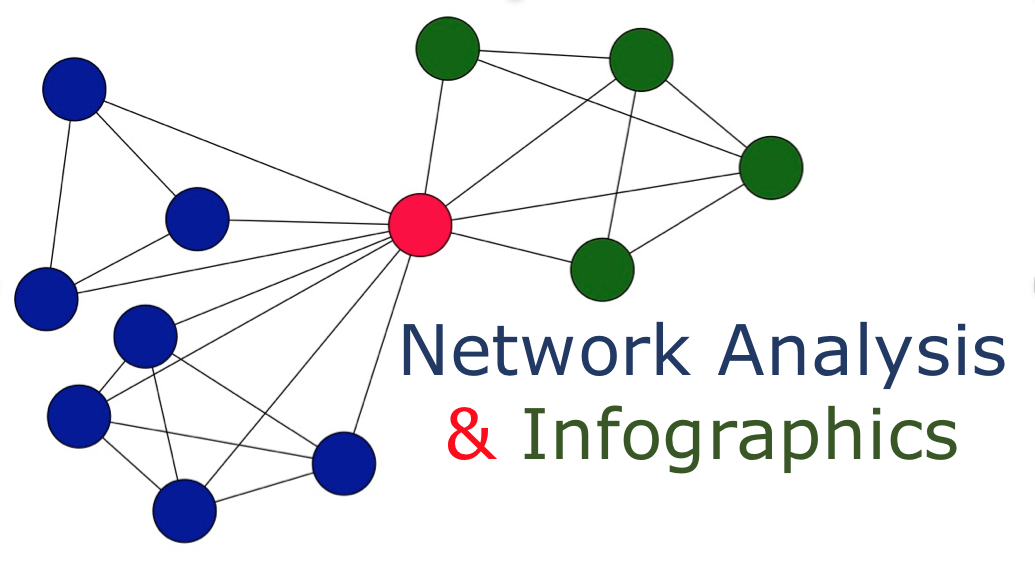
\includegraphics[width=2.5cm]{../_shared_pics/logo}

\medskip

\textit{{\color{dkgreen}{Week 3: 11 February 2022}}}\\
}


\date{} % Date, can be changed to a custom date

\begin{document}

\begin{frame}
\titlepage % Print the title page as the first slide

\begin{textblock*}{10pt}(0pt, 0.9\textheight)

\includegraphics[width=4cm]{../_shared_pics/SPRU.png}
\end{textblock*}

\end{frame}


%=======================================================
%	Learning outcomes
%=======================================================


\begin{frame}
\frametitle{\insertsection}
\framesubtitle{Learning Outcomes}

\centering
\begin{tabular}{lp{5.5cm}l}
\toprule
\multicolumn{2}{l}{\textbf{Learning outcome}} & \textbf{Assessment mode}\\
\hline
\\
1 & 
Explain the concept of network and list the main network indicators & 
ESS\\
\\
\rowcolor{green!20}2 &  
Describe and apply the major techniques for the collection of network data and their statistical analysis & 
ESS, GPN + GWS\\
\\
\rowcolor{green!20}3 & 
Identify the main characteristics of networks by means of network measures  & 
ESS, GPN + GWS\\
\\
4 &
Employ network analysis techniques to produce network data-based infographics & 
GPN + GWS\\
\\
\bottomrule
\multicolumn{3}{l}{\scriptsize Note: ESS: Essay; GPN: Group Presentation; GWS: Group Written Submission}\\
\end{tabular}

\end{frame}

%------------------------------------------------


%=======================================================
%	Intro slides
%=======================================================

\begin{frame}
\frametitle{Overview}
\tableofcontents[hideallsubsections]
\end{frame}

%------------------------------------------------


%=======================================================
%	Introduction to R [recap]
%=======================================================
\section{Introduction to R [recap]}
%------------------------------------------------

\bgroup
\setbeamercolor{background canvas}{bg = navyblue}
\begin{frame}[plain]{}
\begin{center}
\color{white}{\Huge\insertsection}
\end{center}
\end{frame}
\egroup

%------------------------------------------------

\begin{frame}
\frametitle{\insertsection}

\begin{itemize}

\item R creates and manipulate {\color{blue}{objects}}

\medskip

\item Different types or {\color{blue}{classes}} of objects
    \begin{itemize}
    
    \medskip
    
    \item {\color{blue}{Data}} objects 
    	\begin{itemize}
		\item {\color{blue}{vector}}: an ordered collection of values
		\item {\color{blue}{matrix}}: a 2-dimensional vector \\(a vector with $>2$ dimensions is called {\color{blue}{array}})
		\item {\color{blue}{data frame}}: variables and observations
		\item {\color{blue}{list}}: an ordered sequences of objects
		\item {\color{blue}{factor}}: categorical data (e.g.\ ``male'', ``female'')
		\end{itemize}
       
    \medskip
      	  
    \item {\color{blue}{Function}} objects
    		\begin{itemize}
			\item Functions can {\color{blue}{read}}, {\color{blue}{manipulate}} and {\color{blue}{analyse}} data
			\item Packages provide users with {\color{blue}{additional functions}} (e.g.\ igraph)
			\end{itemize}
			
    \end{itemize}

\medskip

\item Objects have {\color{blue}{attributes}}

\item R can read and export a variety of {\color{blue}{data formats}}
\end{itemize}


\end{frame}

%------------------------------------------------

%=======================================================
% Importing/exporting data in R
%=======================================================
\section{Importing/exporting data in R}

%------------------------------------------------

\bgroup
\setbeamercolor{background canvas}{bg = navyblue}
\begin{frame}[plain]{}
\begin{center}
\color{white}{\Huge\insertsection}
\end{center}
\end{frame}
\egroup

%------------------------------------------------

\begin{frame}
\frametitle{\insertsection}

\begin{itemize}[<+->]
\item R can deal with many different data formats
\item Which data formats do you know?
\item Most commonly used data formats
    \begin{itemize}
    \item {\color{blue}{txt}}: fields are usually separated by \textit{comma}, \textit{tab}, \textit{colon}
    \item {\color{blue}{csv}}: fields are separated by \textit{comma}
    \item {\color{blue}{dta}}: format used by STATA to store data
    \item {\color{blue}{xls/xlsx}}: format used by Excel to store data
    \item ...
    \end{itemize}
\item Text editors: Notepad++ (Windows), TextWrangler (Mac)
\item R packages to read and transform data:
    \begin{itemize}
    \item {\color{blue}{``readr''}} (csv, txt, delimited)
    \item {\color{blue}{``readxl''}} (Excel)
    \item {\color{blue}{``haven''}} (STATA, SPSS, SAS)
    \item {\color{blue}{``tidyverse''}}
    \end{itemize}
\item Install these packages in R (you should now know how to do it)
\end{itemize}

\end{frame}

%------------------------------------------------

\begin{frame}
\frametitle{\insertsection}

Let's import/export data in RStudio

\end{frame}

%------------------------------------------------





%=======================================================
%	Network file formats
%=======================================================
\section{Network file formats}
%------------------------------------------------

\bgroup
\setbeamercolor{background canvas}{bg = navyblue}
\begin{frame}[plain]{}
\begin{center}
\color{white}{\Huge\insertsection}
\end{center}
\end{frame}
\egroup

%------------------------------------------------

\begin{frame}
\frametitle{\insertsection}

\footnotesize
\centering
\begin{tabular}{ccccc}
\multicolumn{5}{c}{Composition variables ({\color{blue}{attributes}})}\\
\toprule
Case & Affiliation & Variable $1$ & $\cdots$ & Variable $K$\\
\hline
$1$           \\
$2$           \\
$\vdots$      \\
$N$           \\
\bottomrule
\end{tabular}

\medskip
\medskip
\medskip
\medskip

\footnotesize
\centering
\begin{tabular}{lcccccc}
\multicolumn{7}{c}{Structural variables ({\color{blue}{adjacency matrix}})}\\
\toprule
 &                & \multicolumn{4}{c}{Case}\\
        &        & $1$ & $2$ & $\cdots$ & $N$\\
\hline
        &    $1$           \\
        &    $2$           \\
Case    &    $\vdots$      \\
        &    $N$           \\
\bottomrule
\end{tabular}


\end{frame}

%------------------------------------------------

\begin{frame}
	\frametitle{\insertsection}
	
	
	\centering
	\footnotesize
	\centering
	\begin{tabular}{lccccc}
		\multicolumn{6}{c}{Case-affiliation {\color{blue}{adjacency matrix}}}\\
		\toprule
		&        &\multicolumn{4}{c}{Affiliation}\\
		
		&        & $1$ & $2$ & $\cdots$ & $K$\\
		\hline
		&    $1$           \\
		&    $2$           \\
		Case    &    $\vdots$      \\
		&    $N$           \\
		\bottomrule
	\end{tabular}
	
	
	\medskip
	\medskip
	\medskip
	\medskip
	
	\begin{columns}[c]
		\column{.45\textwidth} 
		\footnotesize
		\centering
		\onslide<2->{\begin{tabular}{lccccc}
				\multicolumn{6}{c}{(1)}\\
				\\
				\multicolumn{6}{c}{Case-case adjacency matrix}\\
				\toprule
				&        &\multicolumn{4}{c}{Case}\\
				
				&        & $1$ & $2$ & $\cdots$ & $N$\\
				\hline
				&    $1$           \\
				&    $2$           \\
				Case    &    $\vdots$      \\
				&    $N$           \\
				\bottomrule
		\end{tabular}}
		
		
		\column{.45\textwidth}
		\footnotesize
		\centering
		\onslide<3->{\begin{tabular}{lccccc}
				\multicolumn{6}{c}{(2)}\\
				\\
				\multicolumn{6}{c}{Affiliation-Affiliation adjacency matrix}\\
				\toprule
				&        &\multicolumn{4}{c}{Affiliation}\\
				
				&        & $1$ & $2$ & $\cdots$ & $K$\\
				\hline
				&    $1$           \\
				&    $2$           \\
				Affiliation    &    $\vdots$      \\
				&    $K$           \\
				\bottomrule
		\end{tabular}}
		
	\end{columns}
	
	
\end{frame}

%------------------------------------------------

\begin{frame}
\frametitle{\insertsection}

\begin{itemize}
\item The variety of {\color{blue}{software packages}} an {\color{blue}{program languages}} has led to a variety of network file formats
    
    \begin{itemize}
    \item GML
    \item GEXF
    \item GDF
    \item GraphML
    \item Pajek NET
    \item GraphViz DOT
    \item UCINET DL
    \item ...
    \end{itemize}

\medskip
\medskip

\item You do not need to remember all these file formats 
    \begin{itemize}
    \item Network file formats are often created from simple {\color{blue}{tables of nodes and edges}}
    \item Most of these formats can be imported in R
    \item New formats are frequently created 
    \end{itemize}

\end{itemize}
\end{frame}

%------------------------------------------------




%=======================================================
%	Introduction to igraph
%=======================================================
\section{Introduction to igraph}
%------------------------------------------------

\bgroup
\setbeamercolor{background canvas}{bg = navyblue}
\begin{frame}[plain]{}
\begin{center}
\color{white}{\Huge\insertsection}
\end{center}
\end{frame}
\egroup

%------------------------------------------------

\begin{frame}
\frametitle{\insertsection}

We focus on:
\begin{itemize}
\item How to create a network
\item How to visualize a network
\item How to add attributes to nodes and edges
\end{itemize}

\end{frame}

%------------------------------------------------

\begin{frame}
\frametitle{\insertsection}

Let's practice this in RStudio (open S3\_R\_Script/S3\_Script.R)

\end{frame}

%------------------------------------------------
 







%%=======================================================
%	Questions
%%=======================================================
\section*{Questions}
%------------------------------------------------

\bgroup
\setbeamercolor{background canvas}{bg = navyblue}
\begin{frame}[plain]{}
\begin{center}
\color{white}{\Huge\insertsection}
\end{center}
\end{frame}
\egroup

%------------------------------------------------





%%=======================================================
%	Next time ...
%%=======================================================
\section*{Next time ...}
%------------------------------------------------

\bgroup
\setbeamercolor{background canvas}{bg = navyblue}
\begin{frame}[plain]{}
\begin{center}
\color{white}{\Huge\insertsection}
\end{center}
\end{frame}
\egroup

%------------------------------------------------

\begin{frame}
\frametitle{\insertsection}

\begin{itemize}
\item 	\textbf{Lecture: Descriptive network analysis A}
	\begin{itemize}
	\item Network measures at the level of the whole network
	\end{itemize}		
	
\medskip
\medskip

\item 	\textbf{Seminar: Descriptive network analysis A}
	\begin{itemize}
	\item Import network data in igraph
	\item Calculate network-level measures in igraph
	\end{itemize}	
		
\end{itemize}

\end{frame}

%------------------------------------------------



\end{document}